\section{The \instname\ data reduction flow.}
\label{sec:reduction_flow}

The spectropolarimetric mode of FORS (PMOS) is enabled by a retarder waveplate (half-wave or quarter-wave retardance between the fast and slow axes) followed by a Wollaston prism (the “analyzer”) which splits the light
beam into two orthogonal polarizations. In order for the two beams not to overlap on the detector, a strip mask
is formed by every second MOS slit jaw carrier arm across the field of view of the instrument as shown in Figure \ref{fig:fors_pmos_data}.

\begin{figure}[h!]
\centering
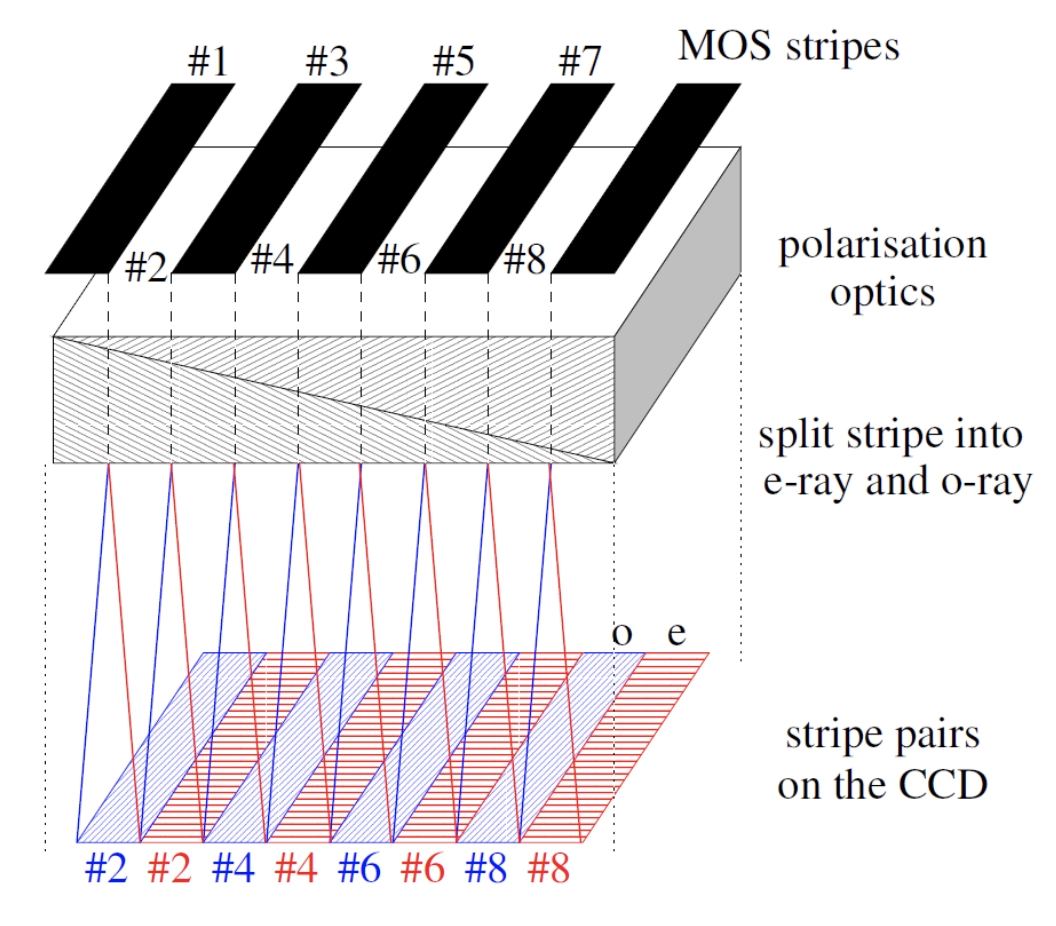
\includegraphics[width=0.9\textwidth]{../instrument_tutorial/figures/fors_pmos_data.jpg}
\caption{Strip mask formed in the focal plane to allow recording of the ordinary o-ray and extraordinary
e-ray beams on the detector. In the even numbered strips, MOS slits can be moved to a particular target position.
For a single point source one strip is sufficient.}
\label{fig:fors_pmos_data}
\end{figure}

The MOS slits can be positioned in the free strips along the dispersion axis to desired target locations.
Frames are recorded at different retarder plate angles in order to allow the computation of the Stokes parameters for the spectra (Bagnulo S., et al., 2009, PASP, 121, 993 7).





The overall data flow of the \instname\ pipeline is displayed in Figure \ref{fig:reduction_cascade}.

 
\begin{figure}[h!]
\centering

\includegraphics[width=0.9\textwidth]{../instrument_tutorial/figures/reduction_cascade.jpg}
\caption{The data reduction cascade of the \instname\ workflow.}
\label{fig:reduction_cascade}
\end{figure}



The reduction cascade is organized in tasks, which represent
well-defined steps in the process. Tasks can be grouped inside
sub-workflows.  Each task runs a recipe; the detailed description of
the algorithms, input, outputs and recipe parameters used in each
recipe are available in the pipeline manual. Here, we present only the
description of most important features.

The \wkfname\  \edps\ workflow is designed to execute the tasks that
deliver the final reduced data cube for each dataset. It can be either
the product of a single exposure, or the combination of multiple
exposures. Only calibrations needed by the selected the scientific
exposures are processed.

It is possible to set \edps\ to perform the data reduction until a
certain step of the reduction chain (e.g. to reduce only standar
stars, or only flat fields).  This is done by specifying the desired
tasks in the field {\bf Select reduction target} of the {\bf Raw Data}
tab.

The reduction steps of the \wkfname\ workflow are listed below. Before
starting the reduction, the parameters of the recipes associated to
each task can be configured by pressing the button

\includegraphics[width=0.8cm]{../common/figures/configure_dataset.jpg}
close to each dataset configuration.
See for more info on the configuration editor \ref{sec:configuration_editor}




\subsection{Creation of the Master Bias}
Task: {\bf bias}  Recipe: {\bf fors\_bias}

In this step the combined MASTER\_BIAS is produced.

The raw bias frames are taken with an exposure time of 0 seconds and a closed shutter. They thus record only the signal
that is added during the read-out of the CCD to avoid negative numbers. A sequence of 5 or 20 raw bias frames is taken the day following the observations as part of the FORS calibration plan (the calibration plan was changed in November 2014; since then 20 bias frames have been taken per setting instead of 5).

Figure \ref{fig:master_bias} shows an example of the quality plot for the MASTER\_BIAS. The image should be uniform, without visible flux gradient. You can also display another extension, IMAGE.ERR for the estimated error per pixel information. See Section \ref{sec:configuration_bias} for more information on how to improve the product if needed.

\begin{figure}[h!]
\centering
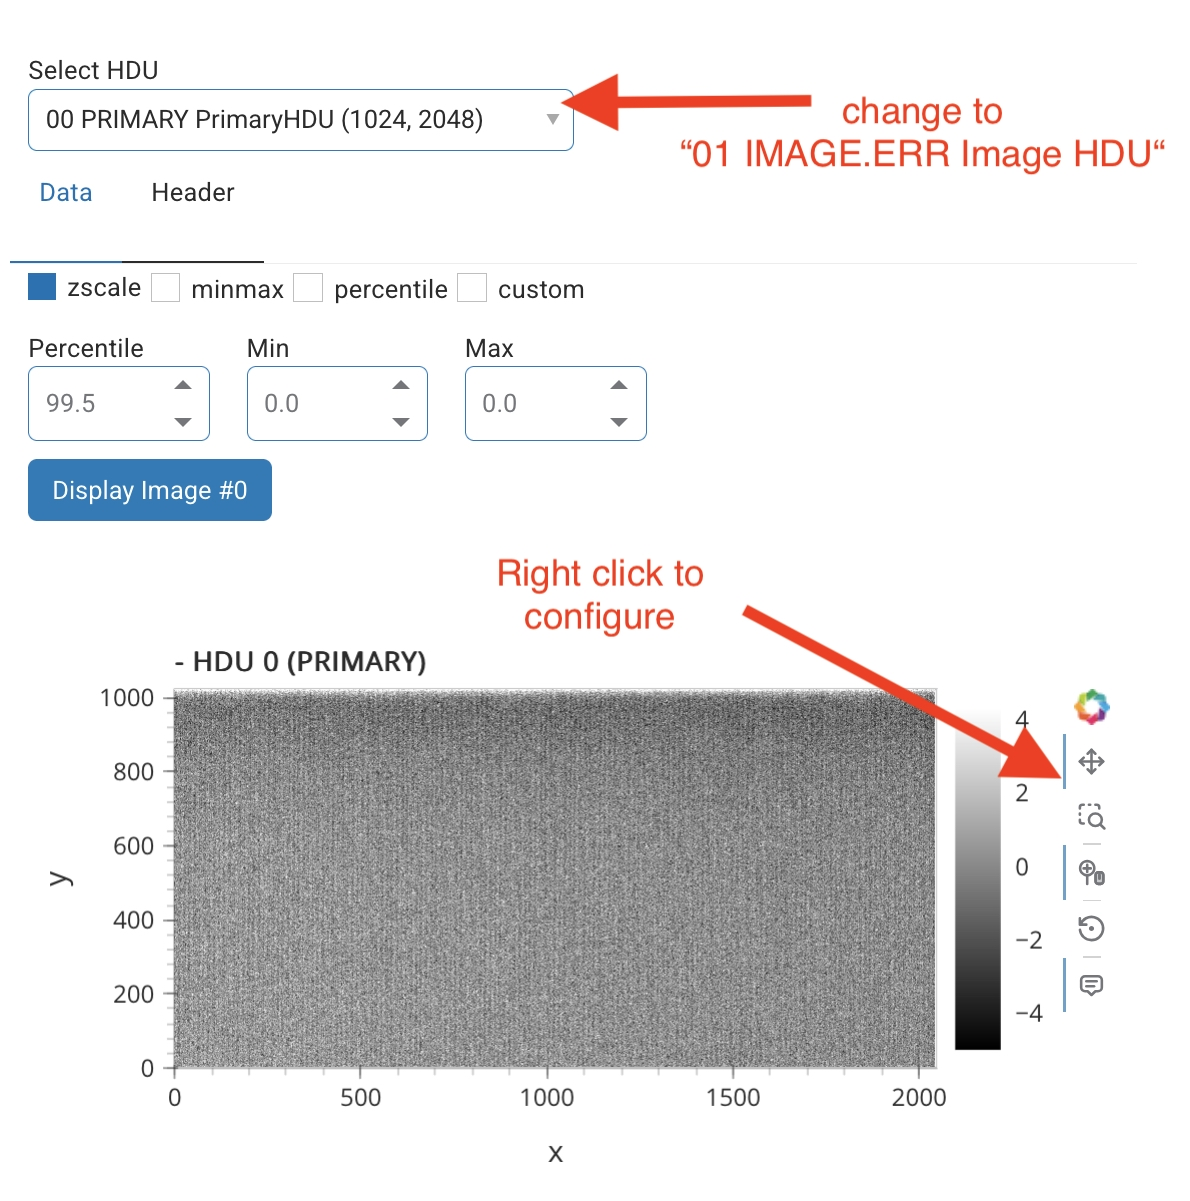
\includegraphics[width=0.9\textwidth]{../instrument_tutorial/figures/master_bias.jpg}
\caption{The quality plot of the MASTER\_BIAS. }
\label{fig:master_bias}
\end{figure}


\subsection{Creating the master Flat Field, determining coefficients for wavelength calibration and correction of spatial distortion}
Task: {\bf calibration\_pmos}  Recipe: {\bf fors\_pmos\_calib}

In this one step, the input screen flat raw calibration frames: SCREEN\_FLAT\_PMOS together with the PMOS arc lamp raw frame: LAMP\_PMOS
are used to create a normalized master flat-field, a 2D dispersion solution, correction for spatial distortion, and to determine the slit limits.

The purpose of the flat-field is to remove the pixel-to-pixel sensitivity variations across the detector. As these
variations act as a noise source, the precision of the flat-field correction will have direct consequences on the
polarimetric precision that can be achieved, and on the signal-to-noise ratio of the reduced observations.
For the spectroscopic modes one will use internal screen flats in most cases. These flats are taken during
daytime with the telescope pointing to zenith and the instrument in calibration position. The flats are taken at
zero retarder plate angle.

For the wavelength calibration the He, HgCd, and Ar lamps (at the lowest spectral resolution with grism 150I) and in addition the Ne lamp (at higher resolution) are used. Wavelength calibration exposures are done
during the day only and at all retarder plate angles used for the science observations.

Products:
\begin{itemize}

\item CURV\_COEFF\_PMOS - table with the coefficients of the spatial curvature fitting polynomials         	
\item CURV\_TRACES\_PMOS - table with the y CCD positions of the detected spectral edges at different x CCD positions.        	
\item DELTA\_IMAGE\_PMOS - deviation from the linear term of the fitting wavelength calibration polynomials. This is a multi-extension FITS file, with one image extension for each input arc lamp exposure.    	
\item DISP\_COEFF\_PMOS - tables with the wavelength calibration polynomial coefficients. This is a multi-extension FITS file, with one table extension for each input arc lamp exposure. Each table contains as
many rows as in the REDUCED\_LAMP\_PMOS images, ordered in the same way.   	
\item DISP\_RESIDUALS\_PMOS - residuals of each wavelength calibration fit (in pixels). These images are only created and inserted in different extensions of a FITS files if the --check configuration parameter is set.
\item DISP\_RESIDUALS\_TABLE\_PMOS - tables containing different kinds of residuals of a sample of wavelength calibration fits. 
\item MAPPED\_NORM\_FLAT\_PMOS - rectified and wavelength calibrated normalised screen flat field image 
\item MAPPED\_SCREEN\_FLAT\_PMOS - rectified and wavelength calibrated master screen flat field image 	
\item MASTER\_NORM\_FLAT\_PMOS - normalised flat field image, derived dividing the master screen flat by its
smoothed version. Comparing this image with the MASTER\_SCREEN\_FLAT\_PMOS may give an immediate feeling of the goodness of the computed curvature model used for the extraction of the normalised spectra.    	
\item MASTER\_SCREEN\_FLAT\_PMOS - combined flat field image. It is the sum of all the input screen flat fields.	
\item REDUCED\_LAMP\_PMOS - rectified and wavelength calibrated arc lamp images, inserted in different extensions of an output FITS file.
\item SLIT\_LOCATION\_PMOS - slit positions, both on the CCD and on the rectified images of the arc lamp exposures (REDUCED\_LAMP\_PMOS).       	
\item SLIT\_MAP\_PMOS - map of central wavelength on the CCD. This image is only created if the --check configuration parameter is set
\item SPATIAL\_MAP\_PMOS - map of spatial positions on the CCD.
\item SPECTRA\_DETECTION\_PMOS - result of the preliminary wavelength calibration applied to the arc lamp exposure. This image is only created if the --check configuration parameter is set.
\item SPECTRAL\_RESOLUTION\_PMOS - Mean spectral resolution for each reference arc lamp line. This is a multi-extension FITS file, with one extension for each input arc lamp frame. 
\item WAVELENGTH\_MAP\_PMOS - map of wavelengths on the CCD. This is a multi-extension FITS file, with one extension for each input arc lamp frame. Each image has the same size of the CCD, where each pixel has the value of the wavelength at its center, if available.    	
\end{itemize}

The important thing in this step is to check the quality of the wavelength
calibration, detection of the slitlets, the flat field combination and normalization.
Figure \ref{fig:master_flat_pmos_1} shows how to examine various products of the fors\_pmos\_calib recipe.

\begin{figure}[h!]
\centering
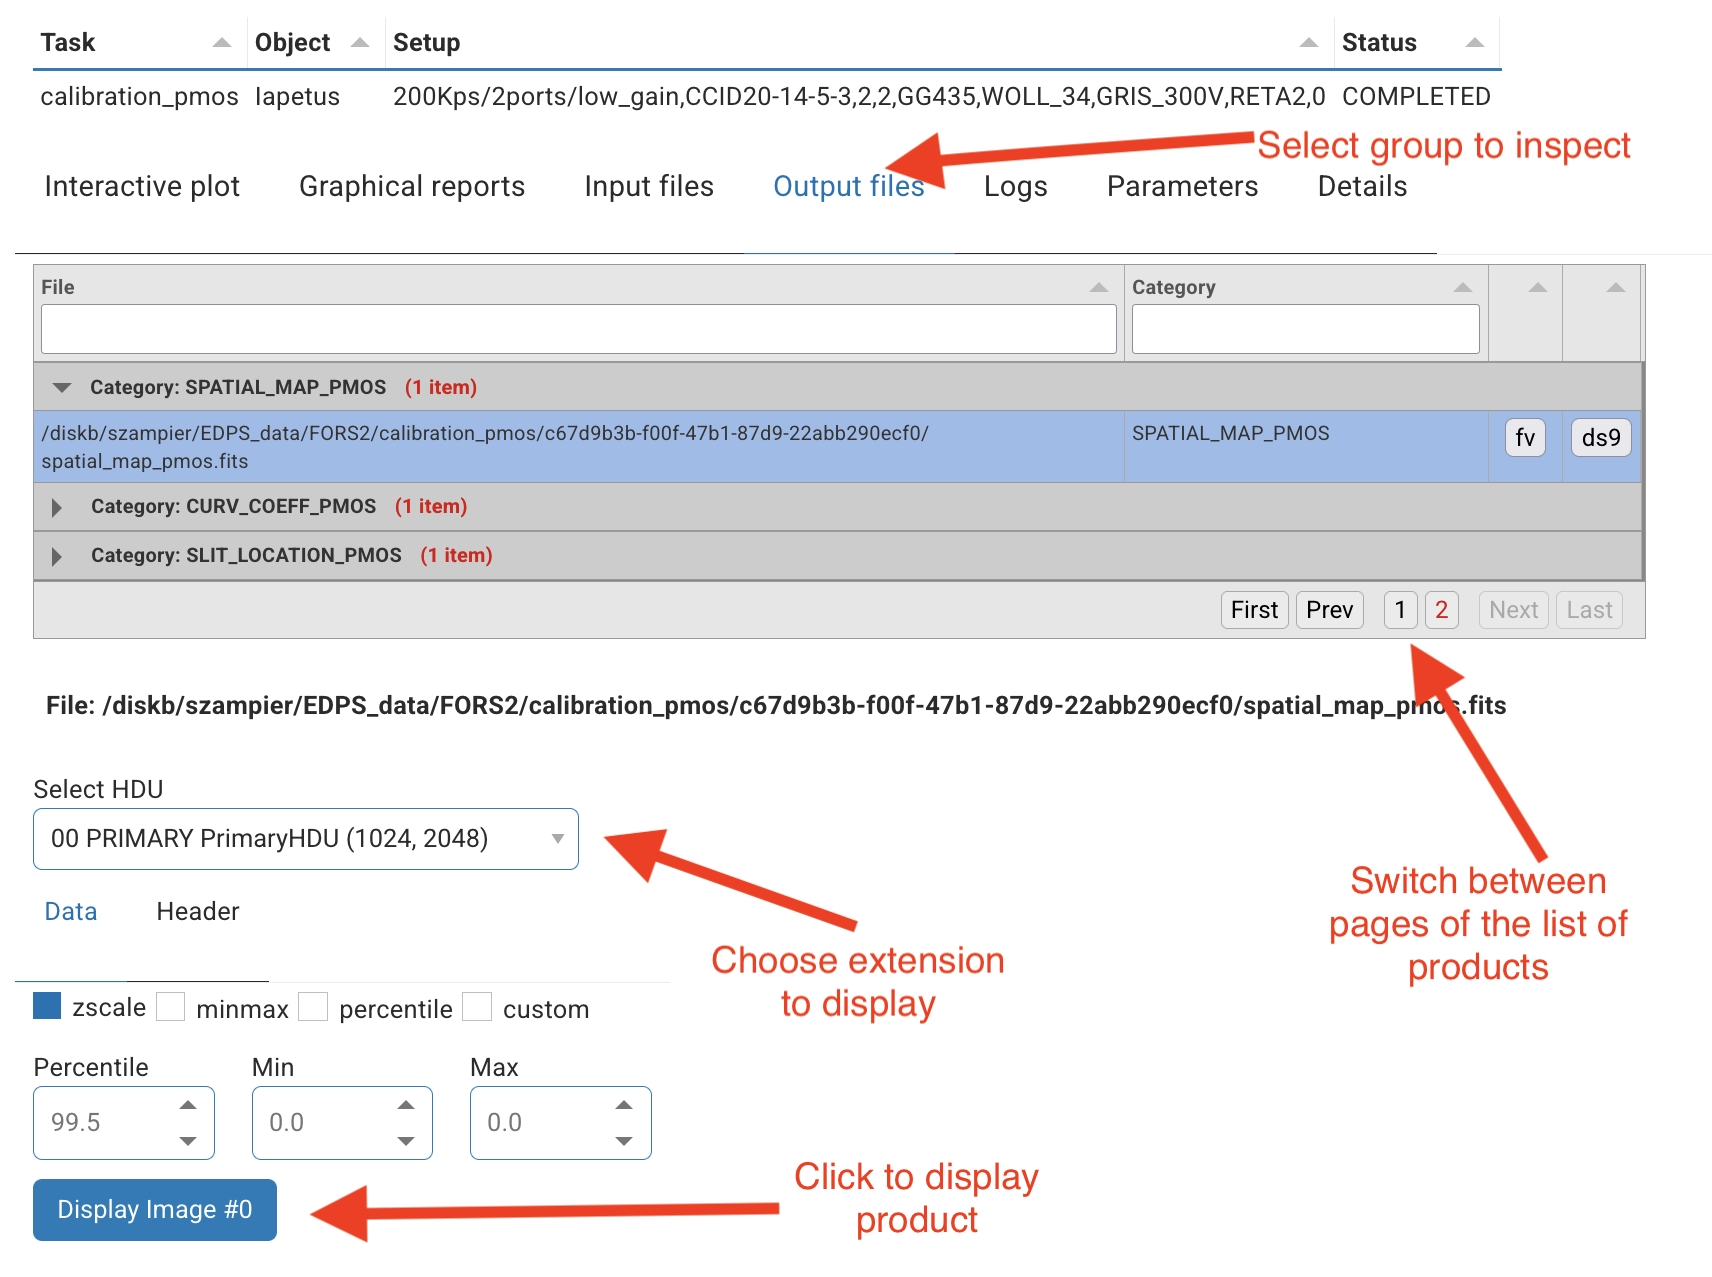
\includegraphics[width=0.9\textwidth]{../instrument_tutorial/figures/master_flat_pmos_1.jpg}
\caption{Examining products of the recipe fors\_pmos\_calib.}
\label{fig:master_flat_pmos_1}
\end{figure}


\begin{figure}[h!]
\centering
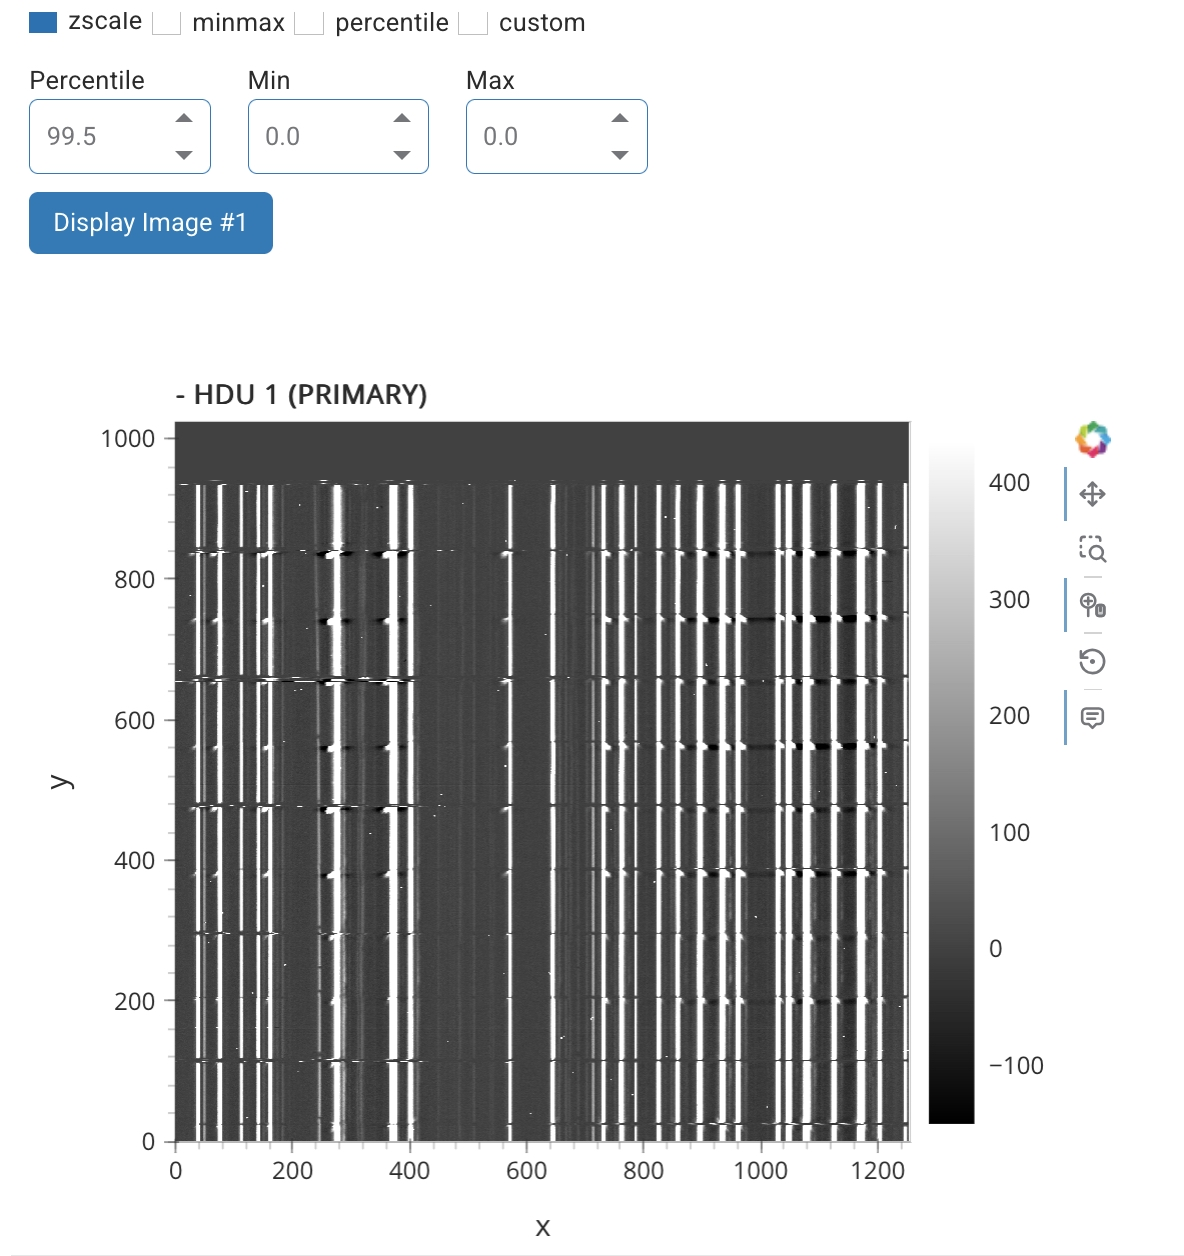
\includegraphics[width=0.9\textwidth]{../instrument_tutorial/figures/master_flat_pmos_2.jpg}
\caption{Example of the SPECTRA\_DETECTION\_PMOS product of the recipe fors\_pmos\_calib.}
\label{fig:master_flat_pmos_2}
\end{figure}

The wavelength calibration can be checked looking at the SPECTRA\_DETECTION\_PMOS product (see Figure \ref{fig:master_flat_pmos_2}). 
In this product the arc lamp lines should run straight from top to
bottom without any empty rows between them. Particular attention should be given to lines at the blue and red ends of each spectrum, where the polynomial fit is more sensitive to small variations of the signal. Some arc lines may show gaps due to the placement of the slits, but empty rows without any lines point towards problems with the detection of the arc lamp lines. See Section \ref{sec:configuration_calibration_pmos} for further information on how to improve the wavelength calibration if necessary.


\begin{figure}[h!]
\centering
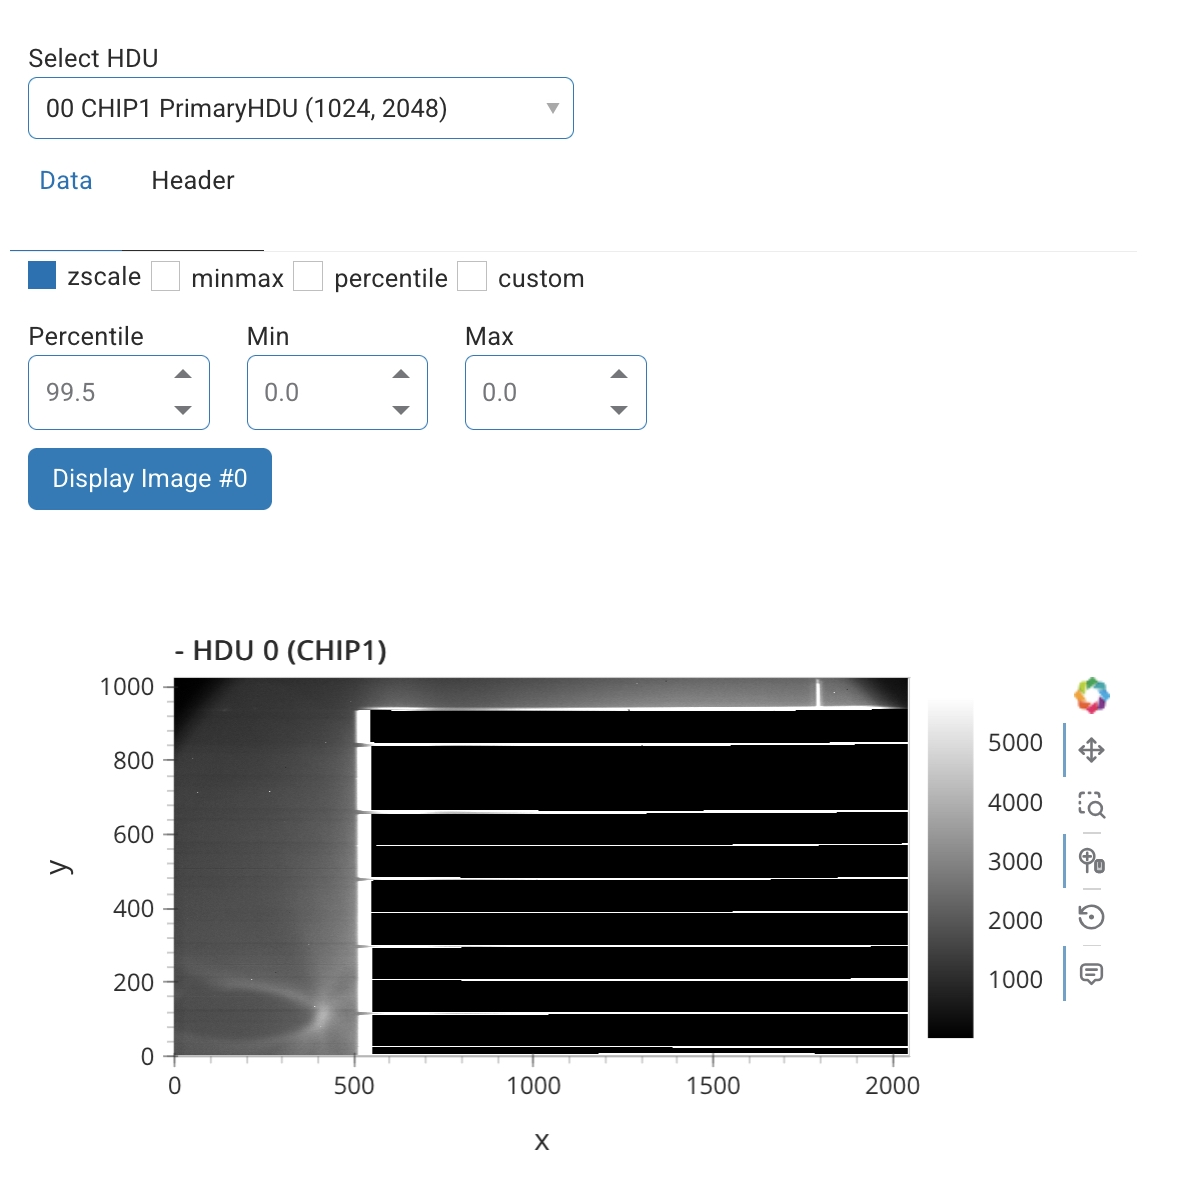
\includegraphics[width=0.9\textwidth]{../instrument_tutorial/figures/master_flat_pmos_3.jpg}
\caption{Example of the MASTER\_NORM\_FLAT\_PMOS product of the recipe fors\_pmos\_calib.}
\label{fig:master_flat_pmos_3}
\end{figure}

The quality of the flat field and detection of the slitlets can be checked inspecting e.g. the SPATIAL\_MAP\_PMOS or the MASTER\_NORM\_FLAT\_PMOS products (see Figure \ref{fig:master_flat_pmos_3}). The spatial map has as pixel values the distance of a pixel from the bottom of the respective slitlet. The regions of the slitlets should not be strongly curved nor should regions of different slitlets overlap with each other. Because all MOS slitlets have similar length the spatial map should show
a similar gradient for all. Note, that it is not the case for the third slitlet from the top. See Section \ref{sec:configuration_calibration_pmos} for tips on how to fix such a problem. All the slitlets should be detected and there should be no spurious detections (e.g. one slitlet detected as several) nor should several
slitlets be detected only as one (as is the case in Figure \ref{fig:master_flat_pmos_3}, see Section \ref{sec:configuration_calibration_pmos}} on how to fix such issue), their edges should be parallel and the areas covered by them should be identical. 

\subsection{Processing Standard Stars and Scientific Observations}

Task: {\bf science\_spectro\_polarimetry} Recipe: {\bf for\_pmos\_science}

In this task the science or the standard star files are processed, applying the calibrations processed in the previous steps. The science files are typically taken at these retarder angles, depending on the desired
level of reduction of systematic error:
\begin{itemize}
\item Circular polarimetry:
\begin{itemize}
\item 2 angles: -45.0, 45.0
\item 4 angles: -45.0, 45.0, 135.0, 225.0
\end{itemize}
\end{itemize}

\begin{itemize}
\item Linear polarimetry:
\begin{itemize}
\item 4 angles: 0.0, 22.5, 45.0, 67.5
\item 8 angles: 0.0, 22.5, 45.0, 67.5, 90.0, 112.5, 135.0, 157.5
\item 16 angles:0.0, 22.5, 45.0, 67.5, 90.0, 112.5, 135.0, 157.5, 180.0, 202.5, 225.0, 247.5, 270.0, 292.5, 315.0, 337.5
\end{itemize}
\end{itemize}

Products:

{\bf 1-dimensional extracted spectra} (*\_REDUCED\_*, created only if spectra are identified and can be extracted).
The individual spectra are provided as rows in a FITS file with as many extensions as input scientific exposures. The correspondence between these rows and the 2-dimensional frames and/or slit identifications
can be obtained from OBJECT\_TABLE\_SCI/STD\_PMOS. All extracted spectra have the same format.
\begin{itemize}
\item REDUCED\_SCI/STD\_PMOS - spectra
\item REDUCED\_ERROR\_SCI/STD\_PMOS - 1 sigma error of spectra
\item REDUCED\_SKY\_SCI/STD\_PMOS - fitted sky spectra
\end{itemize}

{\bf 2-dimensional polarization spectra} (same format as 1-dimensional extracted spectra).
X may be any of ANGLE, I, L, Q, U, V, where V (circular polarisation), Q, U (linear polarisation), L (total linear polarisation, i.e. the
geometrical sum of the Q and U components), ANGLE (direction of the linear polarisation vector in degrees, and finally I (flux in ADU/s). Note that V, Q, U and L are all normalized by I. REDUCED\_ERROR\_SCI/STD\_Q\_PMOS, \_U\_PMOS, \_L\_PMOS, and \_ANGLE\_PMOS are produced when the observation was performed using the half-wave retarder plate, while REDUCED\_ERROR\_SCI/STD\_V\_PMOS is produced when the observation was performed using the 1/4-wave retarder plate. The product REDUCED\_ERROR\_SCI/STD\_I\_PMOS is always produced.
Please note that the polarization parameters U, Q and ANGLE are given with respect to the positive y-axis of the raw data.
\begin{itemize}
\item REDUCED\_X\_SCI/STD\_PMOS - extracted polarisation signals from the object sources.
\item REDUCED\_ERROR\_X\_SCI/STD\_PMOS - 1 sigma errors of the extracted polarisation signals
\item OBJECT\_TABLE\_POL\_SCI/STD\_PMOS - table with position information for detected spectra, with the information from the extensions included within one table.
\end{itemize}

{\bf 2-dimensional wavelength calibrated and distortion corrected frames} (*\_MAPPED\_*, with as many extensions as input scientific exposures)
\begin{itemize}
\item MAPPED\_ALL\_SCI/STD\_PMOS - frame without sky subtraction
\item MAPPED\_SCI/STD\_PMOS - frame, sky-subtracted
\item MAPPED\_SKY\_SCI/STD\_PMOS - frame with fitted sky background
\end{itemize}

If sky alignment is requested (skyalign > 0) the following products are provided in addition to the ones listed above:
\begin{itemize}
\item DISP\_COEFF\_SCI/STD\_PMOS - adjustment of the input DISP\_COEFF\_PMOS table
\item SKY\_SHIFTS\_SLIT\_SCI/STD\_PMOS - table with sky line shifts
\item WAVELENGTH\_MAP\_SCI/STD\_PMOS - wavelength map adjusted for sky line shifts
\end{itemize}


In this step, the quality of the sky subtraction and the spectrum extraction should be checked.

The FORS PMOS pipeline records the 1-dimensional spectra as rows in an image. For the spectroscopic products these images have as many extensions as observed retarder plate angles (=exposures), and each exposure
will create two extracted 1-dimensional spectra per object. The pipeline extracts any signal it finds, so there may be more spectra than intended targets. The extracted polarimetric parameter spectra are stored in single-
extension FITS files, with one row per extracted polarimetric spectrum.

For a typical case of four exposures/retarder angles with only 1 bright target and no other objects the spectroscopic products will have four extensions with two rows each for the two spectra created by the Wollaston prism.
The polarimetric products will have one extension with 1 row.


\begin{figure}[h!]
\centering
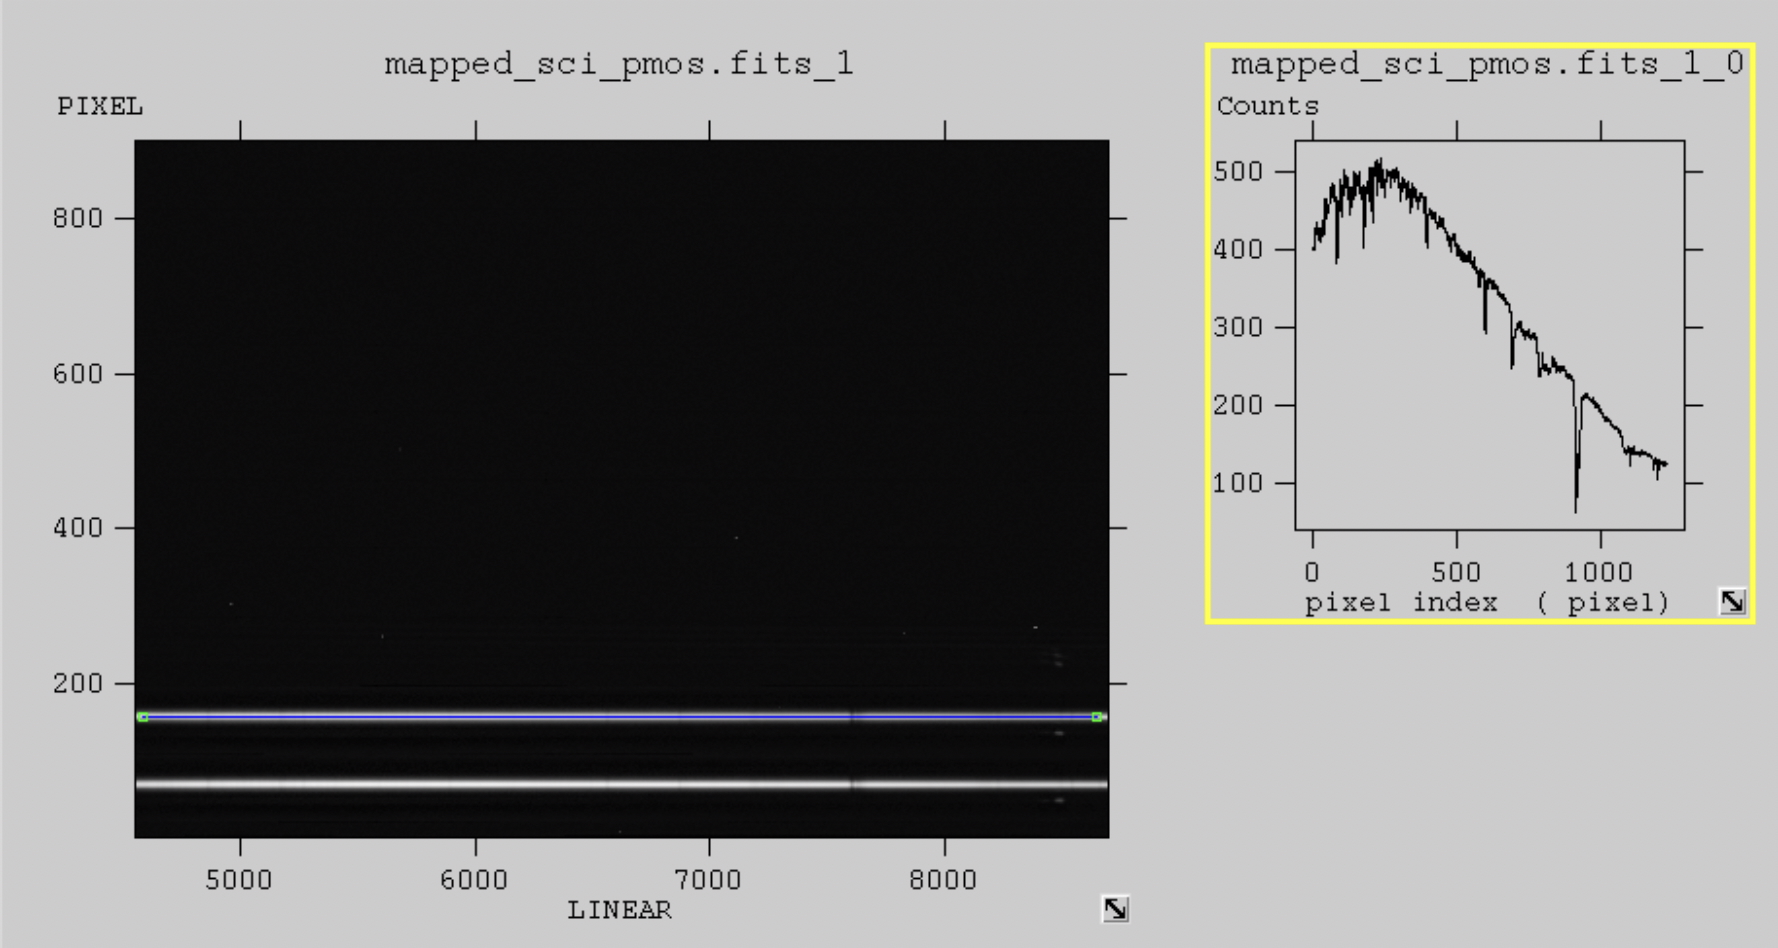
\includegraphics[width=0.9\textwidth]{../instrument_tutorial/figures/mapped_sci_pmos.jpg}
\caption{Example of the mapped sky-subtracted 2-dimensional science product (MAPPED\_SCI\_PMOS) (first exposure only) displayed in fv. The spectrum is in ADU/sec, i.e. not flux-calibrated.}
\label{fig:mapped_sci_pmos}
\end{figure}

Figure \ref{fig:mapped_sci_pmos} shows an example of the mapped sky-subtracted, wavelength-calibrated 2-dimensional spectrum frame (MAPPED\_SCI\_PMOS) (first exposure only) displayed with fv. Every object creates two spectra due to the splitting of the light by the Wollaston prism. The extracted science spectrum should not show strong residuals of sky lines. The spectra
should have a generally smooth look, and will only appear to be noisier in those regions where bright sky lines were subtracted.

The number of extensions corresponds to the number of retarder angles recorded. Please note that there is no one-to-one relation between "extracted spectrum" and "object". For each object there will be two extracted
spectra (one for each light beam). For instance, if a spectro-polarimetric observation consisted of four exposures at four different angles of the retarder plate, each object would have 4 angles x 2 beams = 8 spectra. 

The best way to ensure that the sky was subtracted optimally, at least at the positions of the objects to extract, is to check that the residual noise is compatible with the statistical error associated to the extracted
object spectra. The extracted spectra are contained in the REDUCED\_SCI\_PMOS image (one extracted spectrum for each row). Their error spectra (at a 1-sigma level) are contained in the REDUCED\_ERROR\_SCI\_PMOS
image. The regions of the extracted spectra corresponding to a (bright) sky line will include a few noisier points, which deviation from the spectral continuum should (almost) never pass the 3-sigma deviation.

In some cases the object can have rather low signal, because it was observed by
chance in the same slit as the intended target.

The sky spectra, extracted from the modeled sky frames in exactly the same way as the object spectra from the sky-subtracted frames, can be found in REDUCED\_SKY\_SCI\_PMOS.

Note that if the barycentric correction is applied to the products, the wavelengths are re-computed to match the desired reference system. No interpolation is done on the spectrum itself, only wavelengths are
changed. This means that spectra of the same target might be defined at different wavelengths, depending on the velocity correction. This has to be taken into account when combining spectra for further analysis.


\begin{figure}[h!]
\centering
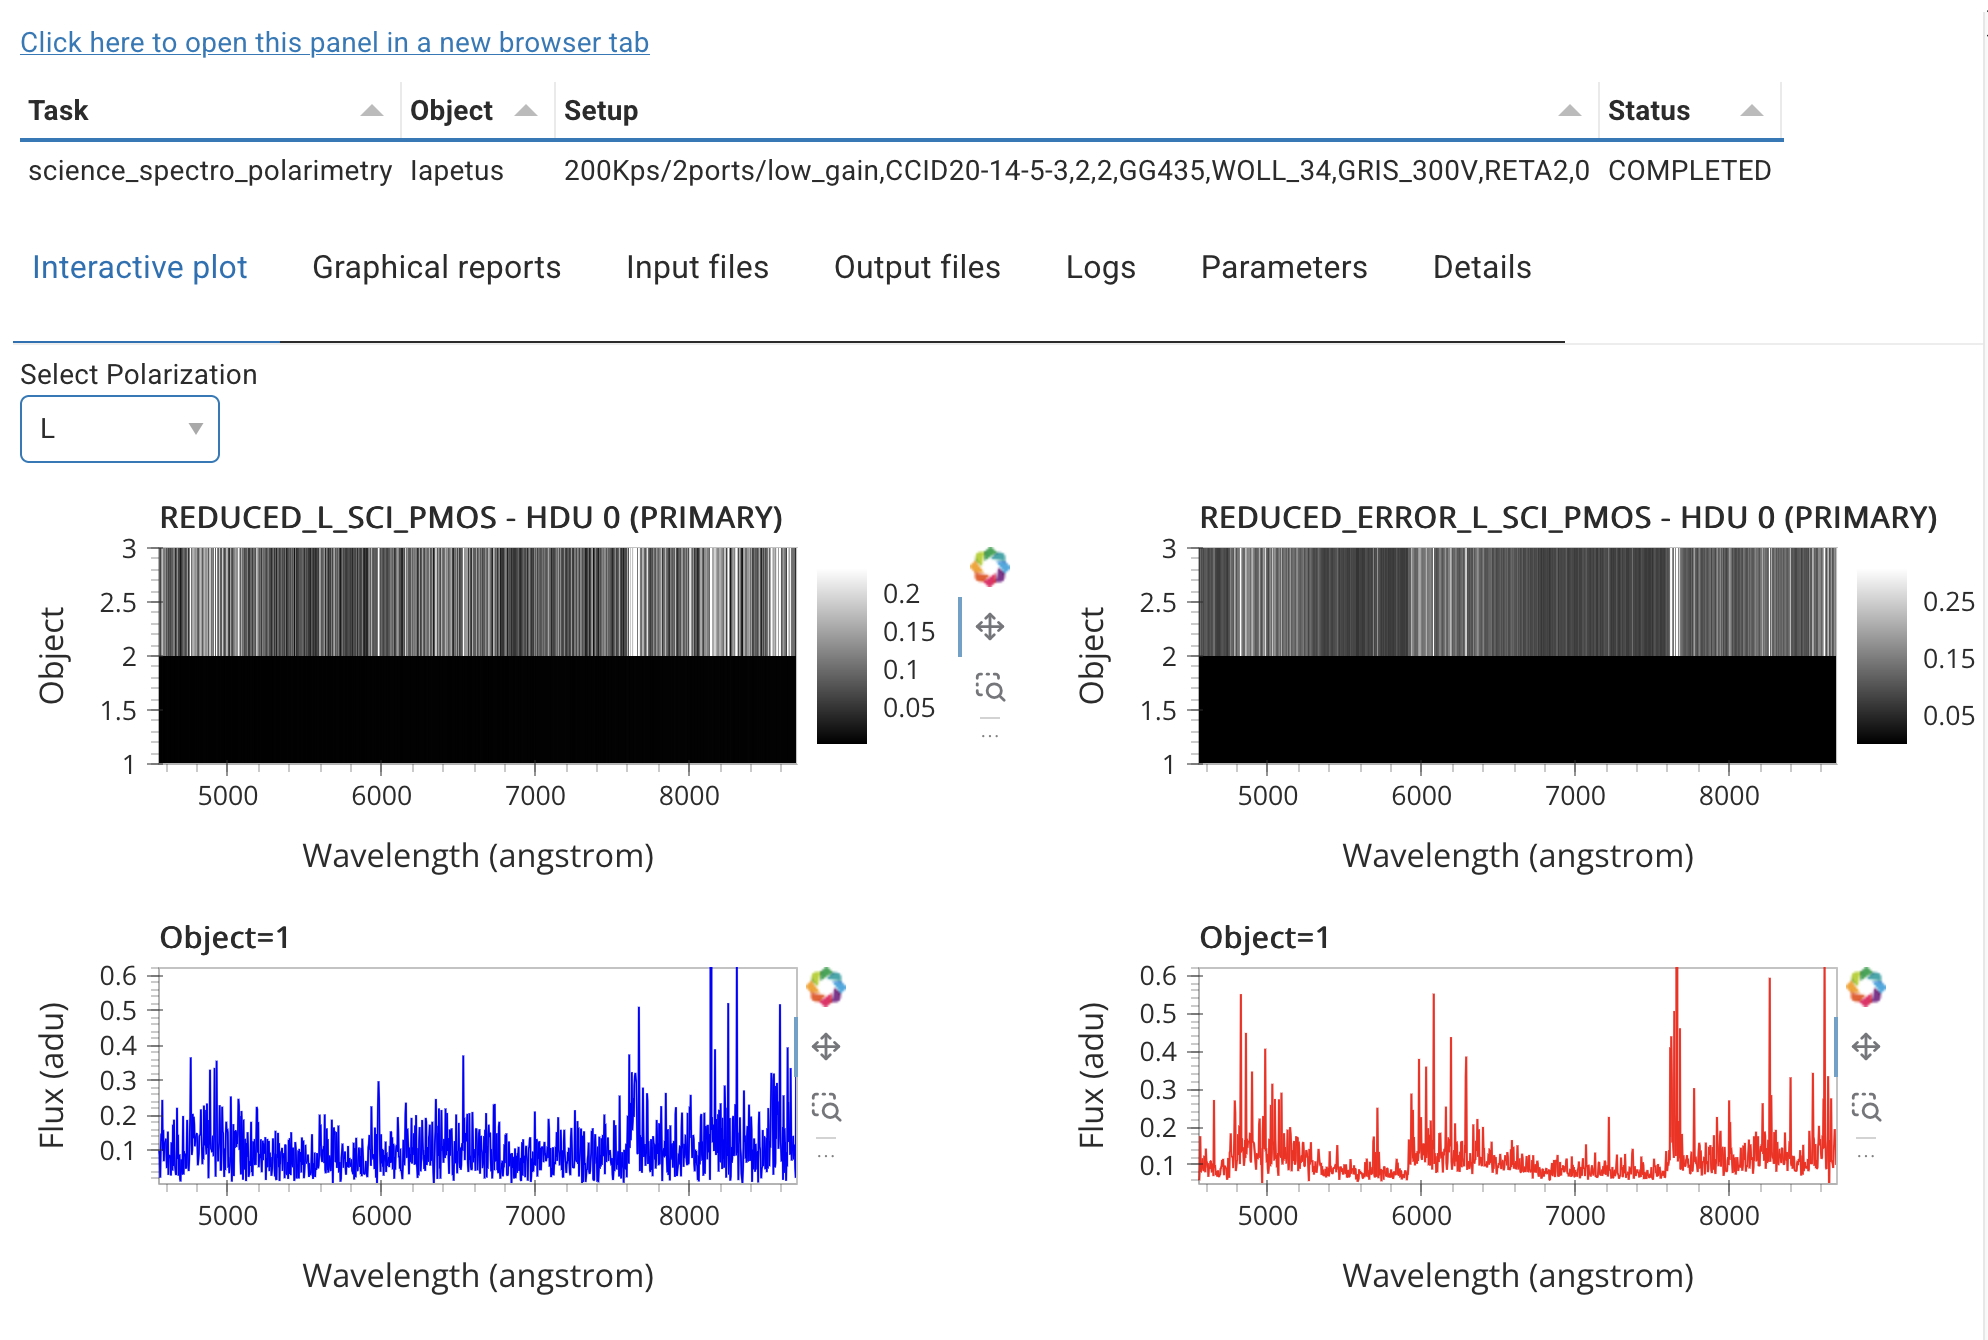
\includegraphics[width=0.9\textwidth]{../instrument_tutorial/figures/interactive_plot_pmos.jpg}
\caption{Example of the Interactive plot for the Task: {\bf science\_spectro\_polarimetry}. It shows the Stokes L (fractional degree of polarization) parameter extracted for the science object (REDUCED\_L\_SCI\_PMOS). The Stokes parameter Q, U, V, and ANGLE can be plotted in the same way via "Select Polarization". Further examination of the "Input files" and the "Output files" can be done by clicking on the corresponding links.}
\label{fig:interactive_plot_pmos}
\end{figure}


The task: {\bf science\_spectro\_polarimetry} Interactive plot (Figure \ref{fig:interactive_plot_pmos}) shows the pipeline determined Stokes L (fractional degree of polarization) parameter of the science object (REDUCED\_L\_SCI\_PMOS). The Stokes Q, U, V, and ANGLE parameter can be displayed as well via the "Select Polarization" menu. In comparison, the REDUCED\_L\_SCI\_PMOS values (top left)  should be higher than the corresponding REDUCED\_ERROR\_L\_SCI\_PMOS values (top right) for the intended science target. 

From here also the "Input files", "Output files", "Logs" etc. can be examined by clicking on the corresponding links.

\subsection{Static calibration data}

In addition to calibration frames taken regularly, the FORS pipeline also uses static calibration tables related to spectropolarimetry. 

\begin{enumerate}
\item Arc lamp line wavelengths (MASTER\_LINECAT). This table contains the reference wavelengths (in Å) for the arc lamp used.
\item Grism table (GRISM\_TABLE). This table contains grism-specific parameters, like the dispersion in Å/pixel,
the start and end wavelength, the polynomial degree to be used for the wavelength calibration, etc.
\item Distortion table (MASTER\_DISTORTION\_TABLE). This table is necessary for the identification of the
ordinary and extraordinary spectral beams.
\item Waveplate chromatism (RETARDER\_WAVEPLATE\_CHROMATISM). This table provides information on
the color dependency of the direction of the linear polarization vector.
\item Polarimetric standard stars catalogue (STD\_PMOS\_TABLE). A table named fors2\_pol\_sta.fits,
listing the measured linear polarisation from a number of standard stars, is available in the calibration
directory.
\end{enumerate}


